\problemname{Laserschack}
Fredrik och Abdullah spelar ett parti Laserschack mot varandra. Spelet spelas på ett rutnät,
och går ut på att skjuta en laserstråle på motståndarens kung.
Abdullah har en attackpjäs som när man trycker på en knapp skjuter ut laser i alla fyra riktningar (upp, ned, höger och vänster), markerad med \texttt{A} i rutnätet.
Fredriks kung är markerad med \texttt{K}. Det finns också spegelpjäser i rutnätet, markerade med \texttt{o}.
När en laser träffar en spegelpjäs studsar strålen ut i all fyra riktningar.

Spelet har just hamnat i en position där Abdullah kommer vinna om han bara trycker på knappen för att skjuta lasern.
För att stoppa Abdullah från att vinna har nu Fredrik lagt ut rökbomber på planen, markerade med \texttt{R}.
Röken stoppar laserstrålar från att färdas genom den rutan. Varje sekund sprider sig röken till alla dom fyra angränsande rutorna.
Om attackpjäsen eller kungen är i rök kan inte Abdullah vinna. 

Hur många sekunder tar det innan Abdullah inte längre vinner genom att trycka på knappen?
Alltså, hur många sekunder tar det tills att röken spridit sig så att lasern inte längre når kungen från attackpjäsen?
Det är garanterat att spelet ursprungligen är i en position där lasern når kungen från attackpjäsen utan att gå genom någon rök.

\section*{Indata}
Den första raden innehåller två heltal $R$ och $C$ ($1\le R, 1 \le C, R\times C \le 250 000$) , antalet rader och kolumner i rutnätet som utgör spelplanen.

De följande $R$ raderna utgör en beskrivning av hur spelplanen ser ut.
Den $i$:te av dessa rader innehåller $C$ tecken som beskriver hur den $i$:te raden ser ut.
Varje tecken är något av följande:
\begin{itemize}
    \item \texttt{.} för en tom ruta
    \item \texttt{o} för en spegelpjäs
    \item \texttt{R} för en rökbomb
    \item \texttt{A} för attackpjäsen
    \item \texttt{K} för kungen
\end{itemize}
Det garanteras att \texttt{A} och \texttt{K} förekommer exakt en gång vardera,
att \texttt{R} förekommer minst en gång,
och att laserstrålen når fram till kungen från attackpjäsen från början.

\section*{Utdata}
Skriv ut ett ickenegativt heltal -- antal sekunder det tar tills lasern inte längre når kungen.

\section*{Poängsättning}
Din lösning kommer att testas på en mängd testfallsgrupper.
För att få poäng för en grupp så måste du klara alla testfall i gruppen.

\noindent
\begin{tabular}{| l | l | l |}
\hline
Grupp & Poängvärde & Gränser \\ \hline
$1$    & $10$       &  $R=1$ \\ \hline
$2$    & $20$       &  Det finns exakt ett \texttt{R} på brädet. \\ \hline
$3$    & $20$       &  Ingen ruta är tom (\texttt{.}) \\ \hline
$4$    & $20$       &  $R\times C \leq 2500$ \\ \hline
$5$    & $30$       &  Inga ytterligare begränsningar. \\ \hline
\end{tabular}

\section*{Förklaring av Exempelfall}
\begin{figure}
  \centering
  \begin{minipage}{.5\textwidth}
    \centering
    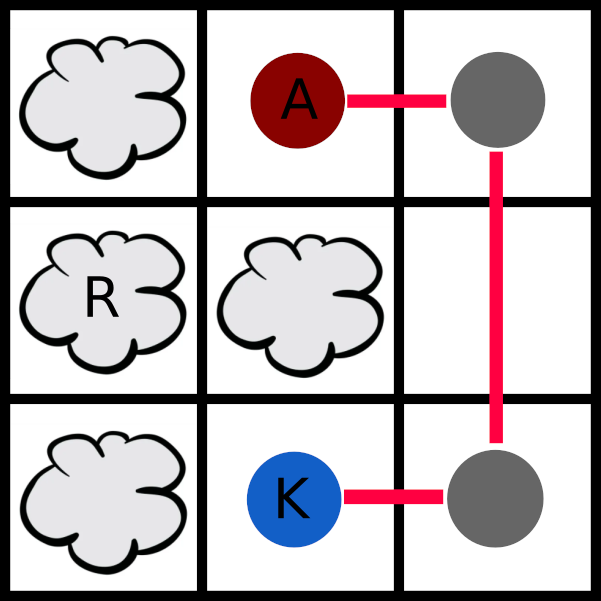
\includegraphics[width=0.5\textwidth]{sample1.png}
    \caption{Sample 1 efter en sekund.}
    \label{fig:test1}
  \end{minipage}%
  \begin{minipage}{.5\textwidth}
    \centering
    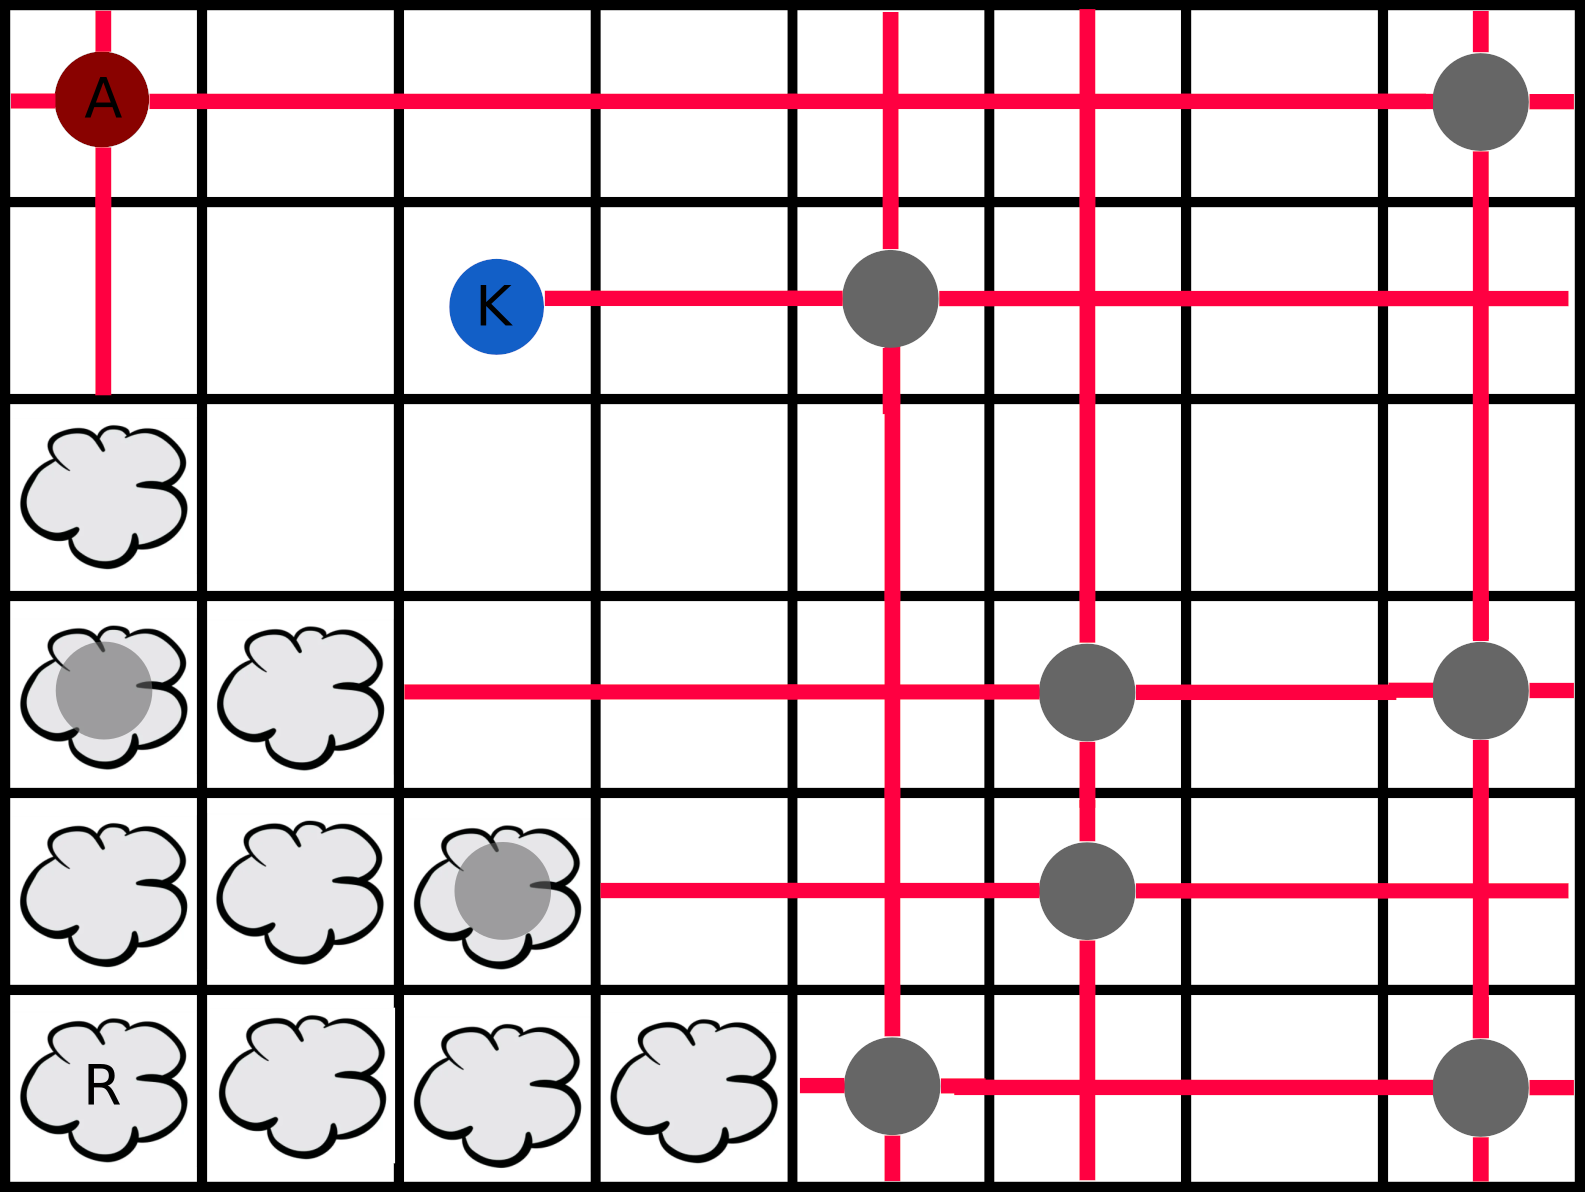
\includegraphics[width=0.8\textwidth]{sample2.png}
    \caption{Sample 2 efter tre sekunder.}
    \label{fig:test2}
  \end{minipage}
\end{figure}
\begin{figure}
    \centering
    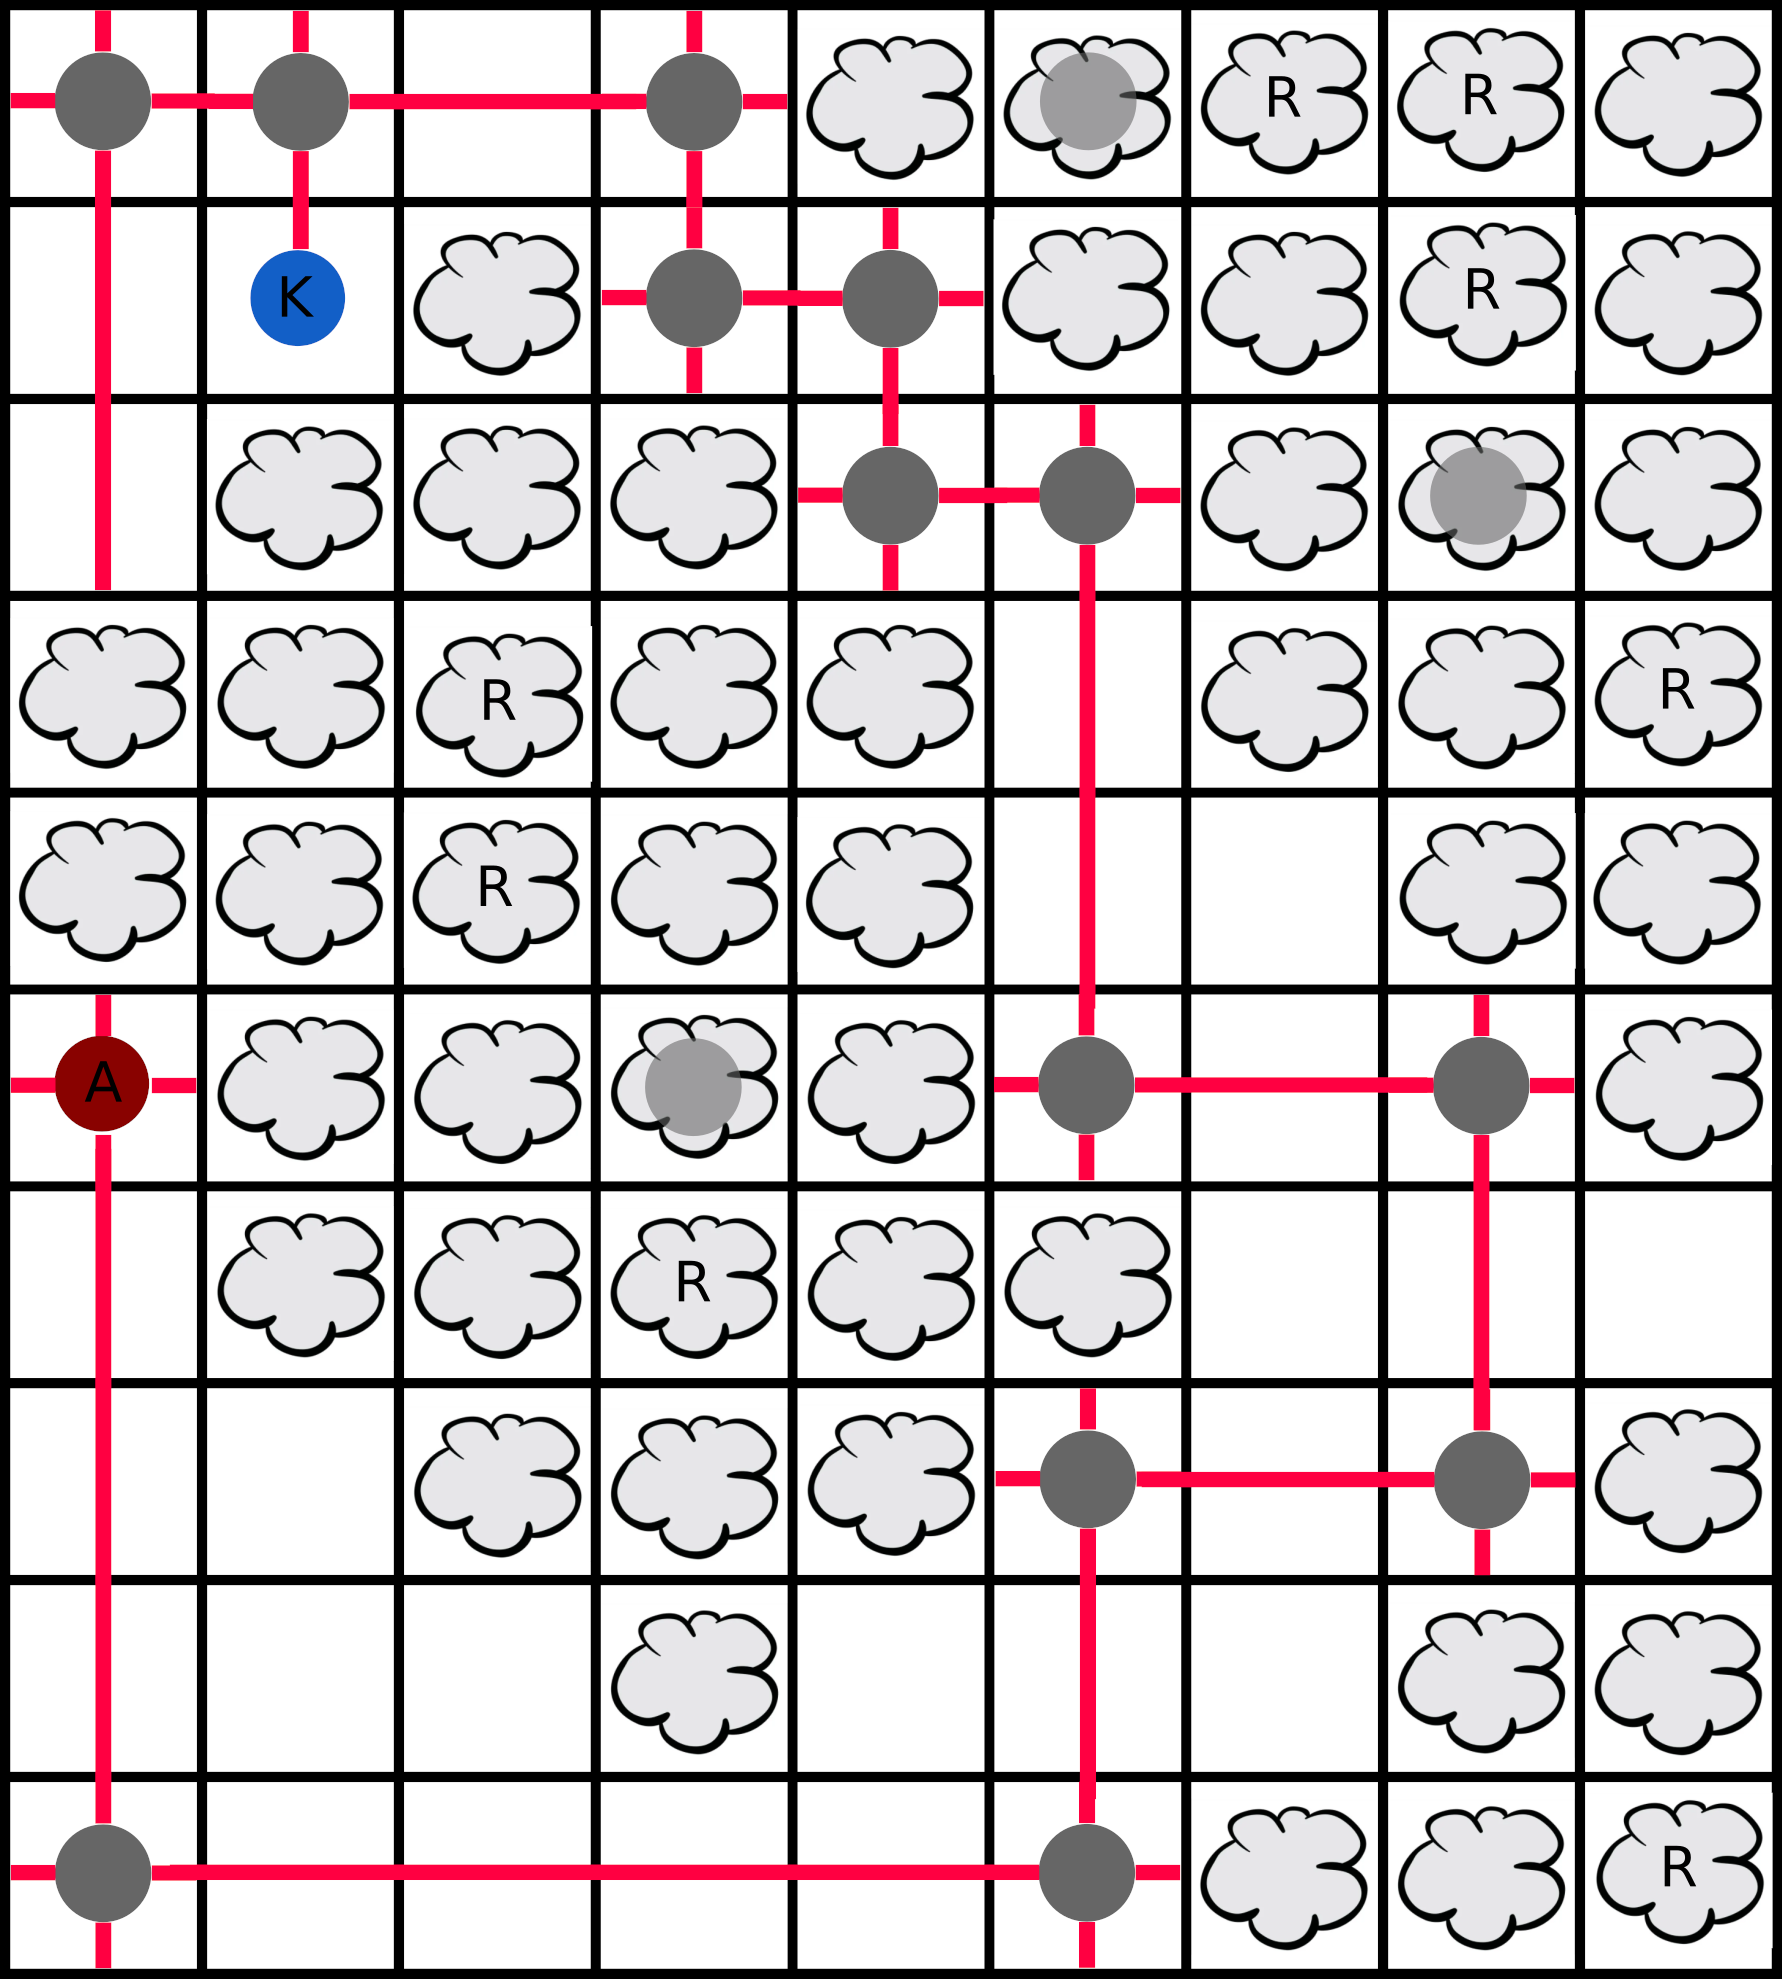
\includegraphics[width=0.5\textwidth]{sample3.png}
    \caption{Sample 3 efter två sekunder.}
    \label{fig:test3}
\end{figure}

Så här ser rökens spridning ut för varje exempelfall i sista sekunden där lasern fortfarande når kungen.

\section*{Exempelfall}
